\documentclass[a4paper, 11pt]{article}
\usepackage{comment} % enables the use of multi-line comments (\ifx \fi) 
\usepackage{fullpage} % changes the margin
\usepackage{graphicx}
\usepackage{fancyvrb,xcolor}
\usepackage{listings}
\usepackage{color}

\definecolor{dkgreen}{rgb}{0,0.6,0}
\definecolor{gray}{rgb}{0.5,0.5,0.5}
\definecolor{mauve}{rgb}{0.58,0,0.82}

\lstset{frame=tb,
  language=Java,
  aboveskip=3mm,
  belowskip=3mm,
  showstringspaces=false,
  columns=flexible,
  basicstyle={\small\ttfamily},
  numbers=none,
  numberstyle=\tiny\color{gray},
  keywordstyle=\color{blue},
  commentstyle=\color{dkgreen},
  stringstyle=\color{mauve},
  breaklines=true,
  breakatwhitespace=true,
  tabsize=3
}
\graphicspath{ {images/} }

\begin{document}
%Header-Make sure you update this information!!!!
\noindent
\large\textbf{Assignment 1} \hfill \textbf{Hussam Hallak} \\
\normalsize CS532, Web Science, Spring 2017\hfill CS Master's Student \\
Computer Science Dept \hfill Prof: Dr. Nelson \\
Old Dominion University \hfill Due Date: 01/26/17

\section*{Question 1:}
Demonstrate that you know how to use ``curl'' well enough to correctly POST data to a form. Show that the HTML response that is returned is ``correct''. That is, the server should take the arguments you POSTed and build a response accordingly. Save the HTML response to a file and then view that file in a browser and take a screen shot.

\subsection*{Answer:}
To post data to a form using ``curl'' command, we need to use the ``-X POST'' option, and then add the option ``-F'' for each ``field=value'' in the form we want to post to.

Example: 

Let's print HTML form a page using ``curl''. This page ``index.html'' is created for test purpose. It makes it possible to post data using a web browser:

\begin{lstlisting}[language=bash]
root@ima-app:/var/www/Hussam# curl http://www.cs.odu.edu/~hhallak/532/A1/Q1/index.html

\end{lstlisting}
Output:
\begin{lstlisting}[language=html]
<html>
<body>

<form action="welcome.php" method="post">
Name: <input type="text" name="name"><br>
E-mail: <input type="text" name="email"><br>
<input type="submit">
</form>

</body>
</html>

\end{lstlisting}
The page ``welcome.php'' expects data to be posted, name and email. Let's see what it looks like without data posted to it. The Superglobal array \$\_POST should be empty:

\begin{lstlisting}[language=bash]
root@ima-app:/var/www/Hussam# curl www.cs.odu.edu/~hhallak/532/A1/Q1/welcome.php   

\end{lstlisting}
Output:
\begin{lstlisting}[language=html]     
<html>
<body>

 Array
(
)

</body>
</html>

\end{lstlisting}

\textbf{Note:}
The code we use to print out the elements of the Superglobal array \$\_POST is what we see if we open ``welcome.php'' in a code editor:

\begin{lstlisting}[language=php]
<html>
<body>
<?php
print_r ($_POST); 
?>
</body>
</html>
\end{lstlisting}

Now it's time to use ``curl'' command to post data to the page ``welcome.php'' and see how it works. The Superglobal array \$\_POST should contain our data that we posted:

\begin{lstlisting}[language=bash] 
root@ima-app:/var/www/Hussam# curl -X POST -F 'name=Hussam' -F 'email=me@hussam.us' http://www.cs.odu.edu/~hhallak/532/A1/Q1/welcome.php

\end{lstlisting}
Output:
\begin{lstlisting}[language=html]
<html>
<body>
 Array
(
    [name] => Hussam
    [email] => me@hussam.us
)
</body>
</html> 

\end{lstlisting}

Now let's save our response to a file. We can easily do that by adding ``-o'' option, and add the name of the file where we want to save the response, to our previous ``curl'' command:
\textbf{Note:}
If the option ``-O'' is used, that is UPPERCASE O, there is no need to add a file name after it; the response will be saved to a file with the same page name.

\begin{lstlisting}[language=bash]
root@ima-app:/var/www/Hussam# curl -X POST -o response.html -F 'name=Hussam' -F 'email=me@hussam.us' http://www.cs.odu.edu/~hhallak/532/A1/Q1/welcome.php

\end{lstlisting}
Output:
\begin{lstlisting} 
  % Total    % Received % Xferd  Average Speed   Time    Time     Time  Current
                                 Dload  Upload   Total   Spent    Left  Speed
100   348    0    97  100   251    999   2586 --:--:-- --:--:-- --:--:--  3691
root@ima-app:/var/www/Hussam# ls
response.html
\end{lstlisting}
We can clearly see that the response is saved to a file named ``response.html''.

\begin{figure}[h]

\caption{Screenshot of The file response.html opened in a web browser}
\centering
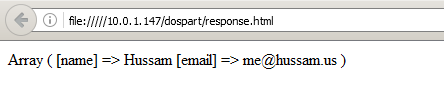
\includegraphics{screen_shot.png}

\end{figure}

\subsection*{Included Files:}
index.html, welcome.php, response.html, screen\_shot.png, session.txt

\section*{Question 2:}
Write a Python program that:
\newline
\indent
1. Takes as a command line argument a web page
\newline
\indent
2. Extracts all the links from the page
\newline
\indent
3. Lists all the links that result in PDF files, and prints out the bytes for each of the links. 
\newline
\indent
(note: be sure to follow all the redirects until the link terminates with a ``200 OK''.)
\newline
\indent
4. show that the program works on 3 different URIs, one of which needs to be:
\newline
\indent
http://www.cs.odu.edu/\textasciitilde mln/teaching/cs532-s17/test/pdfs.html
     
\subsection*{Answer:} 
\lstinputlisting[language=Python]{Q2/extractPDF.py}

\subsection*{Running the program:}
The program takes a link as a command line argument. It follows all the redirects until it terminates with a "200 OK". Then it begins to extract all links to PDF files and prints the PDF link, the final destination for the link, and file size. 

\noindent
\textbf{First Test Case:}

Let's test the link: 
\newline
http://hussam.us 
\newline
The link above is redirected to the link:
\newline
http://www.cs.odu.edu/\textasciitilde hhallak/
\newline
\noindent
This page: http://www.cs.odu.edu/\textasciitilde hhallak/ does not contain any links to PDF documents.
\begin{lstlisting}[language=bash] 
root@ima-app:/var/www/Hussam# python extractPDF.py http://hussam.us
\end{lstlisting}

Output:

\begin{lstlisting}[language=bash]
Entered URL:
http://hussam.us
Final URL:
http://www.cs.odu.edu/~hhallak/
*******************
\end{lstlisting}

\noindent
\textbf{Required Test Case:}

http://www.cs.odu.edu/\textasciitilde mln/teaching/cs532-s17/test/pdfs.html
\begin{lstlisting}[language=bash]

root@ima-app:/var/www/Hussam# python extractPDF.py http://www.cs.odu.edu/~mln/teaching/cs532-s17/test/pdfs.html

\end{lstlisting}

Output:

\begin{lstlisting}[language=bash]
Entered URL:
http://www.cs.odu.edu/~mln/teaching/cs532-s17/test/pdfs.html
Final URL:
http://www.cs.odu.edu/~mln/teaching/cs532-s17/test/pdfs.html
*******************
Extracted link:
http://www.cs.odu.edu/~mln/pubs/ht-2015/hypertext-2015-temporal-violations.pdf
Extracted link final URL:
http://www.cs.odu.edu/~mln/pubs/ht-2015/hypertext-2015-temporal-violations.pdf
Size: 2184076
-------------------------------------
Extracted link:
http://www.cs.odu.edu/~mln/pubs/tpdl-2015/tpdl-2015-annotations.pdf
Extracted link final URL:
http://www.cs.odu.edu/~mln/pubs/tpdl-2015/tpdl-2015-annotations.pdf
Size: 622981
-------------------------------------
Extracted link:
http://arxiv.org/pdf/1512.06195
Extracted link final URL:
https://arxiv.org/pdf/1512.06195.pdf
Size: 1748961
-------------------------------------
Extracted link:
http://www.cs.odu.edu/~mln/pubs/tpdl-2015/tpdl-2015-off-topic.pdf
Extracted link final URL:
http://www.cs.odu.edu/~mln/pubs/tpdl-2015/tpdl-2015-off-topic.pdf
Size: 4308768
-------------------------------------
Extracted link:
http://www.cs.odu.edu/~mln/pubs/tpdl-2015/tpdl-2015-stories.pdf
Extracted link final URL:
http://www.cs.odu.edu/~mln/pubs/tpdl-2015/tpdl-2015-stories.pdf
Size: 1274604
-------------------------------------
Extracted link:
http://www.cs.odu.edu/~mln/pubs/tpdl-2015/tpdl-2015-profiling.pdf
Extracted link final URL:
http://www.cs.odu.edu/~mln/pubs/tpdl-2015/tpdl-2015-profiling.pdf
Size: 639001
-------------------------------------
Extracted link:
http://www.cs.odu.edu/~mln/pubs/jcdl-2014/jcdl-2014-brunelle-damage.pdf
Extracted link final URL:
http://www.cs.odu.edu/~mln/pubs/jcdl-2014/jcdl-2014-brunelle-damage.pdf
Size: 2205546
-------------------------------------
Extracted link:
http://bit.ly/1ZDatNK
Extracted link final URL:
http://www.cs.odu.edu/~mln/pubs/jcdl-2015/jcdl-2015-temporal-intention.pdf
Size: 720476
-------------------------------------
Extracted link:
http://www.cs.odu.edu/~mln/pubs/jcdl-2015/jcdl-2015-mink.pdf
Extracted link final URL:
http://www.cs.odu.edu/~mln/pubs/jcdl-2015/jcdl-2015-mink.pdf
Size: 1254605
-------------------------------------
Extracted link:
http://www.cs.odu.edu/~mln/pubs/jcdl-2015/jcdl-2015-arabic-sites.pdf
Extracted link final URL:
http://www.cs.odu.edu/~mln/pubs/jcdl-2015/jcdl-2015-arabic-sites.pdf
Size: 709420
-------------------------------------
Extracted link:
http://www.cs.odu.edu/~mln/pubs/jcdl-2015/jcdl-2015-dictionary.pdf
Extracted link final URL:
http://www.cs.odu.edu/~mln/pubs/jcdl-2015/jcdl-2015-dictionary.pdf
Size: 2350603
-------------------------------------

\end{lstlisting}

\noindent
\textbf{Additional Test Case:}

http://www.cs.odu.edu/\textasciitilde hhallak/pdfs/index.html

\begin{lstlisting}[language=bash]

root@ima-app:/var/www/Hussam# python extractPDF.py http://www.cs.odu.edu/~hhallak/pdfs/index.html

\end{lstlisting}
Output:
\begin{lstlisting}[language=bash]

Entered URL:
http://www.cs.odu.edu/~hhallak/pdfs/index.html
Final URL:
http://www.cs.odu.edu/~hhallak/pdfs/index.html
*******************
Extracted link:
http://www.cs.odu.edu/~hhallak/pdfs/A4.pdf
Extracted link final URL:
http://www.cs.odu.edu/~hhallak/pdfs/A4.pdf
Size: 191976
-------------------------------------
Extracted link:
http://www.cs.odu.edu/~hhallak/pdfs/cs772A2.pdf
Extracted link final URL:
http://www.cs.odu.edu/~hhallak/pdfs/cs772A2.pdf
Size: 2036216
-------------------------------------
Extracted link:
http://www.cs.odu.edu/~hhallak/pdfs/cs772all.pdf
Extracted link final URL:
http://www.cs.odu.edu/~hhallak/pdfs/cs772all.pdf
Size: 1297575
-------------------------------------
Extracted link:
http://www.cs.odu.edu/~hhallak/pdfs/des-s-boxes.pdf
Extracted link final URL:
http://www.cs.odu.edu/~hhallak/pdfs/des-s-boxes.pdf
Size: 90917
-------------------------------------
Extracted link:
http://www.cs.odu.edu/~hhallak/pdfs/hashes_message_digests.pdf
Extracted link final URL:
http://www.cs.odu.edu/~hhallak/pdfs/hashes_message_digests.pdf
Size: 126965
-------------------------------------
Extracted link:
http://www.cs.odu.edu/~hhallak/pdfs/introduction_authentication.pdf
Extracted link final URL:
http://www.cs.odu.edu/~hhallak/pdfs/introduction_authentication.pdf
Size: 50308
-------------------------------------
Extracted link:
http://www.cs.odu.edu/~hhallak/pdfs/introduction_cryptography.pdf
Extracted link final URL:
http://www.cs.odu.edu/~hhallak/pdfs/introduction_cryptography.pdf
Size: 55243
-------------------------------------
Extracted link:
http://www.cs.odu.edu/~hhallak/pdfs/introduction_general.pdf
Extracted link final URL:
http://www.cs.odu.edu/~hhallak/pdfs/introduction_general.pdf
Size: 26124
-------------------------------------
Extracted link:
http://www.cs.odu.edu/~hhallak/pdfs/introduction_openssl.pdf
Extracted link final URL:
http://www.cs.odu.edu/~hhallak/pdfs/introduction_openssl.pdf
Size: 33765
-------------------------------------
Extracted link:
http://www.cs.odu.edu/~hhallak/pdfs/kerberos.pdf
Extracted link final URL:
http://www.cs.odu.edu/~hhallak/pdfs/kerberos.pdf
Size: 30051
-------------------------------------
Extracted link:
http://www.cs.odu.edu/~hhallak/pdfs/lectures.pdf
Extracted link final URL:
http://www.cs.odu.edu/~hhallak/pdfs/lectures.pdf
Size: 31128
-------------------------------------
Extracted link:
http://www.cs.odu.edu/~hhallak/pdfs/Number Theory.pdf
Extracted link final URL:
http://www.cs.odu.edu/~hhallak/pdfs/Number Theory.pdf
Size: 145137
-------------------------------------
Extracted link:
http://www.cs.odu.edu/~hhallak/pdfs/openssl.pdf
Extracted link final URL:
http://www.cs.odu.edu/~hhallak/pdfs/openssl.pdf
Size: 15481
-------------------------------------
Extracted link:
http://www.cs.odu.edu/~hhallak/pdfs/pem_smime.pdf
Extracted link final URL:
http://www.cs.odu.edu/~hhallak/pdfs/pem_smime.pdf
Size: 36764
-------------------------------------
Extracted link:
http://www.cs.odu.edu/~hhallak/pdfs/PKI_Certificates.pdf
Extracted link final URL:
http://www.cs.odu.edu/~hhallak/pdfs/PKI_Certificates.pdf
Size: 47536
-------------------------------------
Extracted link:
http://www.cs.odu.edu/~hhallak/pdfs/Primes.pdf
Extracted link final URL:
http://www.cs.odu.edu/~hhallak/pdfs/Primes.pdf
Size: 149857
-------------------------------------
Extracted link:
http://www.cs.odu.edu/~hhallak/pdfs/secret_key_cryptography.pdf
Extracted link final URL:
http://www.cs.odu.edu/~hhallak/pdfs/secret_key_cryptography.pdf
Size: 692743
-------------------------------------
Extracted link:
http://www.cs.odu.edu/~hhallak/pdfs/security_handshake.pdf
Extracted link final URL:
http://www.cs.odu.edu/~hhallak/pdfs/security_handshake.pdf
Size: 58099
-------------------------------------
Extracted link:
http://www.cs.odu.edu/~hhallak/pdfs/ssl_https.pdf
Extracted link final URL:
http://www.cs.odu.edu/~hhallak/pdfs/ssl_https.pdf
Size: 49048
-------------------------------------
Extracted link:
http://www.cs.odu.edu/~hhallak/pdfs/ssl_programming.pdf
Extracted link final URL:
http://www.cs.odu.edu/~hhallak/pdfs/ssl_programming.pdf
Size: 52201
-------------------------------------

\end{lstlisting}
\subsection*{Included Files:}
extractPDF.py, README
\newline

\noindent
\textbf{Note:}

The file README contains the following:
\begin{itemize}
\item 
How to use the program
\item 
Required Python version
\item
Required Libraries 
\end{itemize}


\section*{Question 3:}
Consider the ``bow-tie'' graph in the Broder et al. paper (fig 9):
    http://www9.org/w9cdrom/160/160.html

    Now consider the following graph:

    A $\longrightarrow$ B
    
    B $\longrightarrow$ C
    
    C $\longrightarrow$ D
    
    C $\longrightarrow$ A
    
    C $\longrightarrow$ G
    
    E $\longrightarrow$ F
    
    G $\longrightarrow$ C
    
    G $\longrightarrow$ H
    
    I $\longrightarrow$ H
    
    I $\longrightarrow$ K
    
    L $\longrightarrow$ D
    
    M $\longrightarrow$ A
    
    M $\longrightarrow$ N
    
    N $\longrightarrow$ D
    
    O $\longrightarrow$ A
    
    P $\longrightarrow$ G 
    
    For the above graph, give the values for: IN, SCC, OUT, Tendrils, Tubes, Disconnected.

\subsection*{Answer:}
IN: O, M, P
\noindent
\newline
SCC: A, B, C G
\noindent
\newline
OUT: H, D, N
\noindent
\newline
Tendrils: I, K, L
\noindent
\newline
Tubes: there is one tube from M to N (M $\longrightarrow$ N).
\noindent
\newline
Disconnected: E, F
\begin{figure}[h]
\caption{Bowtie graph}
\centering
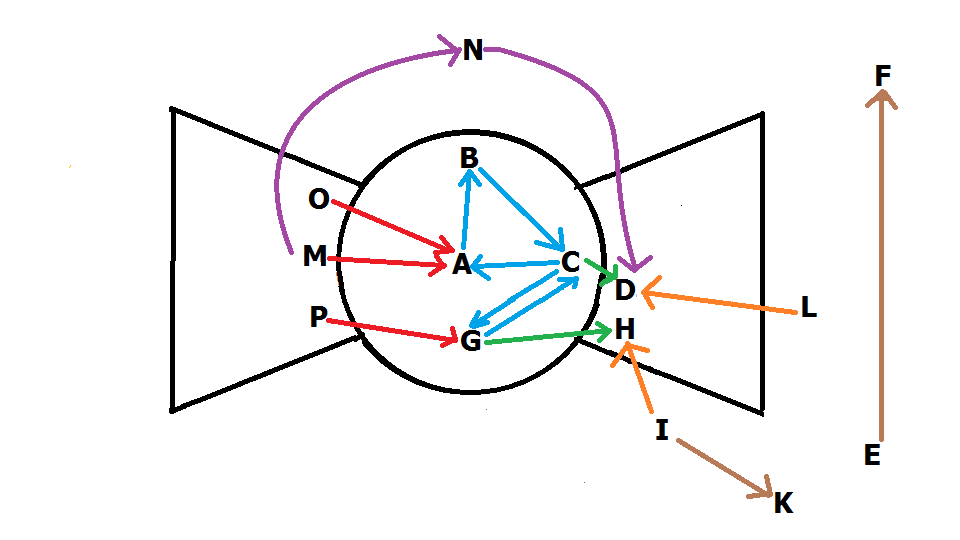
\includegraphics[scale=0.5]{bowtie.png}

\end{figure}[h]
\subsection*{Included Files:}
bowtie.png

\begin{thebibliography}{9}
\bibitem{Python For Beginners} Python For Beginners. Available from World Wide Web:(http://www.pythonforbeginners.com/).
\bibitem{Cambridge University Press} Cambridge University Press. Available from World Wide Web: (http://nlp.stanford.edu/IR-book/html/htmledition/the-web-graph-1.html).
\end{thebibliography}

\end{document}
